\documentclass[12pt, a4paper, twoside, openright]{report}
%\documentclass[12pt, a4paper, twoside, openright]{article}		% 5p gir 2 kolonner pr side. 1p gir 1 kolonne pr side.
\usepackage[T1]{fontenc} 						% Vise norske tegn.
\usepackage[margin=2.5cm]{geometry}
%Options: Sonny, Lenny, Glenn, Conny, Rejne, Bjarne, Bjornstrup
%\usepackage[Bjornstrup]{fncychap}
\usepackage[grey]{quotchap}
% \usepackage[latin1]{inputenc}		% Velger tengsettet i dette dokumentet			
\usepackage[english]{babel}		
\usepackage[utf8]{inputenc}
\usepackage{graphicx}
\usepackage{hyperref}
\usepackage{amsmath,amssymb}
\usepackage{esint}
\usepackage[output-decimal-marker = {,}]{siunitx}
\usepackage[font=footnotesize,labelsep=period,labelfont=bf,margin=1cm]{caption}
\usepackage{import}
\usepackage{caption}
\usepackage{subcaption}
\usepackage{lipsum}
\usepackage{fixmath}
\usepackage[numbers]{natbib}
\usepackage[nottoc,numbib]{tocbibind}
%\usepackage[raggedright]{titlesec}
%\usepackage{titlesec}
\usepackage{emptypage}
%\let\oldsection\section
%\def\section{\cleardoublepage\oldsection}
%\newcommand{\sectionbreak}{\clearpage}
%\usepackage{afterpage}
%\newcommand\blankpage{%
%    \null
%    \thispagestyle{empty}%
%    \addtocounter{page}{-1}%
%    \newpage}
\usepackage{fancyhdr}
\pagestyle{fancy}
\fancyhf{}
\fancyhead[EL]{\nouppercase\leftmark}
\fancyhead[OR]{\nouppercase\rightmark}
\fancyhead[ER,OL]{\thepage}

\setcounter{totalnumber}{5}
\renewcommand{\textfraction}{0.05}
\renewcommand{\topfraction}{0.95}
\renewcommand{\bottomfraction}{0.95}
\renewcommand{\floatpagefraction}{0.35}
\renewcommand{\d}[1]{\ensuremath{\operatorname{d}\!{#1}}}
\DeclareRobustCommand{\orderof}{\ensuremath{\mathcal{O}}}
\setlength\parindent{24pt}
\numberwithin{equation}{chapter}
\numberwithin{figure}{chapter}
\numberwithin{table}{chapter}



\setcounter{totalnumber}{5}
\renewcommand{\textfraction}{0.05}
\renewcommand{\topfraction}{0.95}
\renewcommand{\bottomfraction}{0.95}
\renewcommand{\floatpagefraction}{0.35}

\makeatletter
\def\ps@pprintTitle{%
  \let\@oddhead\@empty
  \let\@evenhead\@empty
  \let\@oddfoot\@empty
  \let\@evenfoot\@oddfoot
}
\makeatother

\begin{document}

\begin{titlepage}

\newcommand{\HRule}{\rule{\linewidth}{0.5mm}} % Defines a new command for the horizontal lines, change thickness here

\center % Center everything on the page
 
%----------------------------------------------------------------------------------------
%	HEADING SECTIONS
%----------------------------------------------------------------------------------------

%\textsc{\LARGE Norwegian University of \\ \vspace{0.3cm} Science and Technology}\\[1.5cm] % Name of your university/college
\textsc{\Large Master thesis in applied physics and mathematics}\\[0.5cm] % Major heading such as course name
%\textsc{\large Minor Heading}\\[0.5cm] % Minor heading such as course title

%----------------------------------------------------------------------------------------
%	TITLE SECTION
%----------------------------------------------------------------------------------------

\HRule \\[0.4cm]
%{ \huge \bfseries The dynamics of skyrmions in an electric field}\\[0.4cm] % Title of your document
{ \huge \bfseries Control of skyrmion motion via current and inhomogeneous electric fields in thin-film Dzyaloshinskii-Moriya ferromagnets with Rashba spin-orbit coupling}\\[0.4cm]
\HRule \\[1.5cm]
 
%----------------------------------------------------------------------------------------
%	AUTHOR SECTION
%----------------------------------------------------------------------------------------

\begin{minipage}{0.4\textwidth}
\begin{flushleft} \large
\emph{Author:}\\
\O yvind \textsc{Johansen} % Your name
\end{flushleft}
\end{minipage}
~
\begin{minipage}{0.4\textwidth}
\begin{flushright} \large
\emph{Supervisor:} \\
Prof. Jacob \textsc{Linder} % Supervisor's Name
\end{flushright}
\end{minipage}\\[4cm]

% If you don't want a supervisor, uncomment the two lines below and remove the section above
%\Large \emph{Author:}\\
%John \textsc{Smith}\\[3cm] % Your name

%----------------------------------------------------------------------------------------
%	DATE SECTION
%----------------------------------------------------------------------------------------

{\large \today}\\[3cm] % Date, change the \today to a set date if you want to be precise

%----------------------------------------------------------------------------------------
%	LOGO SECTION
%----------------------------------------------------------------------------------------

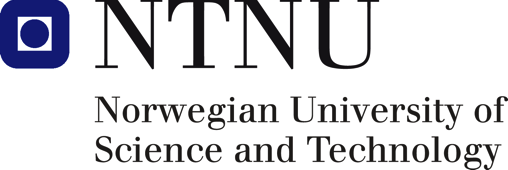
\includegraphics[width=0.5\textwidth]{Figures/ntnu-logo.png} % Include a department/university logo - this will require the graphicx package
 
%----------------------------------------------------------------------------------------

\vfill % Fill the rest of the page with whitespace

\end{titlepage}

%\title{Magnetization dynamics of domain walls and skyrmions in micromagnetics}
%\author{\O yvind Johansen}
%\date{\today}

%\maketitle
%\afterpage{\blankpage}
\pagenumbering{roman}

\chapter*{Abstract}
\addcontentsline{toc}{chapter}{Abstract}
\newpage

\chapter*{Sammendrag}
\addcontentsline{toc}{chapter}{Sammendrag}
\newpage

\chapter*{Preface}
\addcontentsline{toc}{chapter}{Preface}
%\\

\begin{minipage}{0.95\textwidth}
\begin{flushright}
\O yvind Johansen \\
Trondheim, Norway \\ 
2016
\end{flushright}
\end{minipage}\\[4cm]

\newpage

\tableofcontents

\newpage
%\afterpage{\blankpage}

\pagenumbering{arabic}

\chapter{Introduction}

\chapter{Fundamental theory}
%\section{Zeeman energy}
%The Zeeman energy is the energy contribution from the interaction between the magnetization $\mathbold{M}(\mathbold{r})$ in the magnetic material and an external magnetic field $\mathbold{H}_Z(\mathbold{r})$. This energy can be expressed as
%\begin{align}
%E_Z = -\mu_0\int \d V \mathbold{M}(\mathbold{r})\cdot\mathbf{H}_Z(\mathbold{r}),
%\end{align}
%with $\mu_0$ being the vacuum permeability.
\section{Energy terms in micromagnetics}
\subsection{Exchange energy}
Ferromagnetism occurs in materials where the spins tend to align with each other, and thereby being able to generate an observable magnetic field outside of the material. The mechanism behind this is the exchange interaction between the spins. In ferromagnetic materials the system can lower its energy by having parallel neighboring spins. This is described by the Heisenberg Hamiltonian,
\begin{align}
H = - J\sum_{\langle i,j\rangle} \mathbold{S}_i\cdot\mathbold{S}_j,
\end{align}
with $J$ being the exchange integral which is positive for ferromagnetic materials and $\mathbold{S}$ a dimensionless spin-vector. The spins can be expressed in terms of the magnetization, which is the average magnetic moment. As the magnetic moment and the spin of an electron are anti-parallel, this relation becomes
\begin{align}
\mathbold{S}_i = -\frac{S}{M_s}\mathbold{M}_i,
\end{align}
with $M_s$ being the saturation magnetization and $S$ the magnitude of the spin. The magnetization is a classical vector, and in micromagnetism it is treated as a slowly varying smooth function. One can therefore perform a Taylor expansion of it. By doing that, one can show \cite{Project} that the energy density can be written as
\begin{align}
\epsilon_{EX} = \frac{\textrm{d} E_{EX}}{\textrm{d} V} = -\frac{A}{M_s^2}\mathbold{M}(\mathbold{r})\mathbold{\nabla}^2\mathbold{M}(\mathbold{r}) = \frac{A}{M_s^2}\partial_i\mathbold{M}(\mathbold{r})\partial_i\mathbold{M}(\mathbold{r}), \label{eq:exchDensity}
\end{align}
with $A$ being the exchange stiffness
\begin{align}
A = \frac{J S^2}{2a}
\end{align}
and $a$ being the lattice constant.
\subsection{Perpendicular magnetic anisotropy}
In some magnetic materials we may have something known as magnetic anisotropy. As the name indicates, there is an anisotropy in the material that makes certain magnetization directions more energetically favorable than others. This mostly stems from the spin-orbit coupling. If one considers the restframe of the electron instead of the proton, the proton is orbiting the electron and thereby causing a temporal varying electric field. Amp\`{e}re's ciruital law then says that the electron observes a magnetic field proportional to the orbital motion of the proton. This magnetic field then interacts with the magnetic moment of the electron, which is proportional to the spin, hence the name spin-orbit coupling. Taking this into consideration as well as the atomic structure in the material, one can see that one could end up with a material where the magnetic field the electrons experience from the spin-orbit coupling would allow one direction to be easier magnetized than others.

In some layered ultrathin film structures, such as Pd/Co \cite{Carcia1985}, it has been discovered that the magnetization has a lower energy when it is perpendicular to the films. This means that the easy axis of the material is perpendicular to the films, and we then have something called perpendicular magnetic anisotropy (PMA). The anisotropic energy is independent of the direction the magnetization has along the easy axis, meaning the energy is the same if the magnetization points into or out of the films. Letting $K$ be the anisotropy constant and $\theta$ the angle to the normal of the films, the anisotropic energy density can then be written as
\begin{align}
\epsilon_{PMA} = K\sin^2\theta \label{eq:PMADensity}
\end{align} 
to the lowest order in $\theta$. Here we have normalized the energy density in such a way that if the magnetization points along the easy axis the energy density is zero.

\subsection{Voltage induced magnetic anisotropy} \label{sec:VIMA}
One form of perpendicular magnetic anisotropy occurs at the interface between certain materials. This has been attributed to the exchange interaction between $p-$ and $d-$oribitals at material interfaces, such as the 3$d$ orbital in Fe and 2$p$ orbital in O at an Fe/MgO interface \cite{Matsukura2015}. As this is a magnetic anisotropy that only occurs at the surface of the material, it will only be of importance in ultra-thin magnetic films where surface effects are of a greater importance. It has also been discovered that one can modify the strength of this surface magnetic anisotropy with an external electric field. The reason for the change of strength in the magnetic anisotropy is the modification of the occupation number in the 3$d$ orbitals in Fe, thereby affecting the $p-d$ exchange interaction that is the origin of the magnetic surface anisotropy \cite{Maruyama2009}. It was found that in a thin-film system with an Fe/MgO interface where the Fe layer consisted of only a few monoatomic layers a change of approximately 40\% could be achieved in the magnetic surface anisotropy by application of an external electric field. As it is relatively easy to generate a localized electric field, one can therefore create an energy landscape to influence the dynamics of magnetization patterns. An example of this was shown by Uphadhyaya et al. by guiding dipole-dipole interaction skyrmions with voltage gates \cite{Upadhyaya2015}.

\subsection{Rashba spin-orbit coupling}
In materials where the motion of the electrons is confined to a plane, and the inversion symmetry is broken along the axis perpendicular to that plane, there is a splitting of the spin energy levels. Inversion symmetry can for example be broken at the interface between two materials \cite{Heide2006}. The inversion asymmetry causes an electric field perpendicular to the plane of motion, as the gradient of the electrostatic potential becomes non-zero when inversion symmetry is broken ($V(\mathbold{r}) \neq V(-\mathbold{r})$). When particles move in an electric field, they experience a magnetic field which can be seen by performing a Lorentz transformation into the particles' restframe. This magnetic field is proportional to $\mathbold{v}\times\mathbold{E}$. Because of the magnetic field the energy levels become spin dependent, as the field couples to the spin. This is described by the Rashba Hamiltonian \citep{BychovRashba1984}
\begin{align}
H_R &= \frac{\alpha_R}{\hbar}\mathbold{\sigma}\cdot(\mathbold{p}\times\mathbold{\hat{n}}) = \alpha_R (\mathbold{\sigma}\times\mathbold{k})\cdot\mathbold{\hat{n}}.
\label{eq:RashbaH}
\end{align}
Here $\alpha_R$ is the Rashba parameter, $\mathbold{p} = \hbar\mathbold{k}$ the momentum of the electrons, $\mathbold{\hat{n}}$ a unit vector perpendicular to the plane of motion and $\mathbold{\sigma}$ is a vector of the Pauli matrices.

\subsection{The Dzyaloshinskii--Moriya interaction}
The Dzyaloshinskii--Moriya interaction (DMI) is an antisymmetric exchange coupling between spins, given by the Hamiltonian
\begin{align}
H_{DM} = \sum_{\langle i,j\rangle}\mathbold{D}_{ij}\cdot(\mathbold{S}_i\times\mathbold{S}_j). \label{eq:DMIHamiltonian}
\end{align}
This interaction only occurs in materials where the inversion symmetry is broken. The magnitude of $\mathbold{D}_{ij}$ depends on the material properties, and the direction of $\mathbold{D}_{ij}$ depends on the symmetry of the atomic structure in the material. Moriya showed \cite{Moriya1960} that if there is an $n$-fold axis (with $n \geq 2$) along the axis between the particles with spins $\mathbold{S}_i$ and $\mathbold{S}_j$, $\mathbold{D}_{ij}$ will be parallel to that axis. Using that in a Taylor expansion of \eqref{eq:DMIHamiltonian}, it can be shown that the energy density becomes
\begin{align}
\epsilon_{DM}^{\textrm{(bulk)}} = \frac{D}{M_s^2}\mathbold{M}\cdot(\mathbold{\nabla}\times\mathbold{M}).
\end{align}
On the other hand, if there is a mirror plane located at the center of the line between the particles with spins $\mathbold{S}_i$ and $\mathbold{S}_j$ that is perpendicular to the axis intersecting them, the vector $\mathbold{D}_{ij}$ lies in the mirror plane. In a more specific case where the interaction between the spins $\mathbold{S}_i$ and $\mathbold{S}_j$ is mediated by a third magnetic particle (different from the other two) located in the mirror plane, $\mathbold{D}_{ij}$ is perpendicular to the triangle spanned by the three particles as illustrated in Figure \ref{fig:InterfacialDMI}. Assuming the magnetic particles with spins $\mathbold{S}_i$ and $\mathbold{S}_j$ are located in the $xy$-plane, and that the mediating magnetic particle of a different type lies above them, a Taylor expansion of \eqref{eq:DMIHamiltonian} yields the energy density
\begin{align}
\label{eq:DMInterface}
\epsilon_{DM}^{\textrm{(interface)}} = \frac{D}{M_s^2}\left[M_z(\mathbold{\nabla}\cdot\mathbold{M})-(\mathbold{M}\cdot\mathbold{\nabla})M_z\right].
\end{align}
\begin{figure}[h!]
\begin{center}
\includegraphics[width=0.6\textwidth]{Figures/InterfacialDMI.pdf} 
\caption{An illustration of the geometry of an interfacial DMI. The antisymmetric interaction between the spins $\mathbold{S}_i$ and $\mathbold{S}_j$ is mediated by a third magnetic particle in blue. The direction of $\mathbold{D}_{ij}$ is then perpendicular to the plane spanned by the three particles.}
\label{fig:InterfacialDMI} 
\end{center}
\end{figure}
The observant reader may have noticed that both the Rashba spin-orbit coupling and Dzyaloshinskii-Moriya interaction occur in materials with inversion asymmetry. Dzyaloshinskii first introduced DMI based on a phenemenological reasoning \citep{Dzyaloshinskii1958} to describe what had been observed experimentally, and Moriya later proposed that the microscopic mechanism behind this was spin-orbit coupling \cite{Moriya1960}. In thin-film system it is then reasonable to assume that Rashba spin-orbit coupling can be the mechanism behind DMI. This was in fact shown mathematically by Kim \textit{et al.} \citep{DMIfromRashba_Kim}. They started with the model Hamiltonian
\begin{align}
H = H_{\textrm{kin}} + H_R + H_E = \frac{\mathbold{p}^2}{2m_e} + \frac{\alpha_R}{\hbar}\mathbold{\sigma}\cdot(\mathbold{p}\times\mathbold{\hat{n}}) + J\mathbold{\sigma}\cdot\mathbold{\hat{M}}
\end{align}
that includes the kinetic energy of electrons confined to a plane, a Rashba spin-orbit coupling and the symmetric exchange energy between the spins. A unitary transformation was then performed on the Hamiltonian to remove the explicit Rashba Hamiltonian from the model, so that the transformed Hamiltonian could be written as $H' = U^{\dagger} H U = H_{\textrm{kin}} + H_E' + \orderof(\alpha_R^2)$. This unitary transformation, defined by
\begin{align}
U = \exp\left[-i\frac{\alpha_R m_e}{\hbar^2}\mathbold{\sigma}\cdot(\mathbold{r}\times\mathbold{\hat{n}})\right],
\end{align}
does not change the eigenvalues of the system, and the physics in the transformed Hamiltonian is therefore the same as the original model Hamiltonian. It was then shown that the transformed symmetric exchange energy included an interfacial DMI term with the strength of the parameter $D$ being
\begin{align}
D = \frac{4\alpha_Rm_e A}{\hbar^2}.
\end{align}

\section{Skyrmions}
In certain types of materials, such as chiral magnets, an exotic magnetization pattern has been found to occur. This magnetization pattern, known as a skyrmion, is a vortex-like magnetization structure with non-trivial topology. The magnetization of the skyrmion wraps around the unit sphere, meaning that it has a non-zero skyrmion number \cite{Heinze2011}
\begin{align}
\label{eq:SkyrmionNumber}
N_{\textrm{sk}} = \frac{1}{4\pi}\int \mathbold{\hat{M}}\cdot(\partial_x \mathbold{\hat{M}} \times \partial_y \mathbold{\hat{M}}) \d x \d y.
\end{align}
Skyrmions have an integer skyrmion number, while vortices have a half-integer skyrmion number \cite{Tretiakov2007}. The magnetization of the skyrmion can be written in cartesian coordinates as
\begin{align}
\label{eq:SkyrmionMVec}
\mathbold{M}(\rho, \phi) = M_s
\begin{pmatrix}
\cos\Phi(\phi)\sin\theta(\rho) \\ \sin\Phi(\phi)\sin\theta(\rho) \\ \cos\theta(\rho)
\end{pmatrix}.
\end{align}
As the out-of-plane component (here the $z$-component) of the magnetization in the skyrmion is rotationally symmetric around the skyrmion's core, the out-of-plane angle $\theta$ can be written as a function of $\rho$ only, with $\rho$ being the distance to the skyrmion's core. The in-plane magnetization angle $\Phi$ is assumed to be a linear function of the azimuthal angle $\phi$, such that
\begin{align}
\Phi = m\phi + \psi.
\end{align}
Due to the periodical nature of the angles, $m$ is constrained to be an integer. The phase difference $\psi$ between $\Phi$ and $\phi$ is a constant called the helicity of the skyrmion. If one plugs in the ansatz \eqref{eq:SkyrmionMVec} into \eqref{eq:SkyrmionNumber}, one finds that
\begin{align}
N_{\textrm{sk}} = \frac{m}{4\pi}\int_0^{2\pi}\d\phi \int_0^{\infty}\d \rho \sin\theta(\rho) \frac{\partial\theta(\rho)}{\partial\rho} = - \frac{m}{2} \cos(\theta(\rho))|_{(\rho = 0)}^{(\rho=\infty)}.
\end{align}
Unless $m$ is an even number, one must require that $\theta(\rho = 0) = 0$ and $\theta(\rho = \infty) = \pi$, or $\theta(\rho = 0) = \pi$ and $\theta(\rho = \infty) = 0$ for the skyrmion number to be an integer and not a half-integer.

The skyrmion needs a certain type of physical mechanism in the material to be a stable state. This mechanism will allow a lower energy state by having the neighbouring spins not be entirely parallel to each other, like the symmetric exchange interaction wants them to be. One of these mechanisms is the Dzyaloshinskii--Moriya interaction, which is the stabilizing mechanism of skyrmions we will consider in this thesis. Other mechanisms that can also cause the magnetic skyrmion to be a stable state are long-ranged magnetic dipolar interactions \cite{Lin1973}, frustrated exchange interactions \cite{Okubo2012} and four-spin exchange interactions \cite{Heinze2011}. If we consider the interfacial DMI energy density in \eqref{eq:DMInterface} and plug in our ansatz for the magnetization of the skyrmion, one finds that
\begin{align}
\epsilon_{DM}^{\textrm{(interface)}} = D\cos((m-1)\phi + \psi)\left(\frac{\partial\theta}{\partial\rho} + \frac{m}{\rho}\sin\theta\cos\theta\right).
\end{align}
For the DMI to have a net energy contribution, we must remove the dependence on $\phi$ as the average of a harmonic function over the plane will be zero. We therefore require that $m = 1$, which is not an even number, meaning we must apply the boundary conditions for $\theta(\rho)$ mentioned earlier. The helicity $\psi$ is then chosen to minimize the energy contribution from DMI, which leaves us with the two options $\psi = 0$ and $\psi = \pi$, depending on the sign of $D$ and the $\theta$ profile. Due to the boundary conditions for $\theta$, the magnetization in the core of the skyrmion points in the opposite direction of the magnetization far away from the skyrmion core. The magnetization direction far away from the core must therefore be a stable direction in the energy. This can be done in a system with an easy axis parallel to that direction. If we consider a skyrmion in a thin film, which makes sense with our choice of interfacial DMI, the easy axis must be perpendicular to that film. In other words, we need a thin-film system with perpendicular magnetic anisotropy. Finally, as our system is ferromagnetic, we also need to include the symmetric exchange interaction. This is also necessary if we want to treat the skyrmion in the micromagnetic model, where we assume that the magnetization can be estimated by a smooth function. This assumption was for example used in the Taylor expansion of the DMI Hamiltonian. Our model then has the energy density given by
\begin{align}
\nonumber \epsilon &= \epsilon_E + \epsilon_{PMA} + \epsilon_{DM}^{\textrm{(interface)}} \\
&=A \left[\left(\frac{\partial\theta}{\partial\rho}\right)^2 + \frac{\sin^2\theta}{\rho^2}\right] + K\sin^2\theta + D\cos\psi\left(\frac{\partial\theta}{\partial\rho} + \frac{1}{\rho}\sin\theta\cos\theta\right),
\end{align}
assuming a magnetization profile given by \eqref{eq:SkyrmionMVec}. The energy is independent of $\phi$ due to our choice of $m$, but it remains a function of $\theta$ and $\rho$. As the skyrmion is a ground state, we can find the function $\theta(\rho)$ by minimizing the energy. Using the condition
\begin{align}
\frac{\delta\epsilon(\theta, \rho)}{\delta\theta(\rho)} = \frac{\partial\epsilon}{\partial\theta} - \frac{\textrm{d}}{\textrm{d}\rho} \frac{\partial\epsilon}{\partial (\frac{\partial\theta}{\partial \rho})} = 0
\end{align}
and introducing the dimensionless length $\tilde{\rho} = \rho D/A$, one ends up with the following differential equation for $\theta(\rho)$:
\begin{align}
\label{eq:ODEtheta}
\frac{\partial^2\theta}{\partial\tilde{\rho}^2} + \frac{1}{\tilde{\rho}}\frac{\partial\theta}{\partial\tilde{\rho}} - \frac{\sin\theta\cos\theta}{\tilde{\rho}^2}+\cos\psi\frac{\sin^2\theta}{\tilde{\rho}}-\frac{AK}{D^2}\sin\theta\cos\theta = 0.
\end{align}
Definining the ratio $AK/D^2$ as a parameter $C$, one can solve this equation numerically for a given $C$. Some numerical solutions are shown in Figure \ref{fig:ThetaProfile} when the boundary conditions $\theta(\rho = 0) = \pi$ and $\theta(\rho = \infty)$ have been used. It should be noted that this differential equation only has a solution when $\cos\psi = 1$ for the chosen boundary conditions. The solutions for the different helicities $\psi_1 = 0$ and $\psi_2 = \pi$ have a simple relation, however. This relation can be verified to be
\begin{align}
\theta_{\psi_1}(\rho) = \pi - \theta_{\psi_2}(\rho),
\end{align}
as $\cos\psi$ is antisymmetric under a swap in helicities, and $\frac{\partial^2\theta}{\partial\tilde{\rho}^2}$, $\frac{\partial\theta}{\partial\tilde{\rho}}$, $\cos\theta_{\psi_i}$ are all antisymmetric under the relation above.
\begin{figure}[h!]
\begin{center}
\includegraphics[width=0.6\textwidth]{Figures/SkyrmionRadialProfiles.pdf} 
\caption{The solution of the out-of-plane angle $\theta$ of the skyrmion profile for different values of $C$.}
\label{fig:ThetaProfile} 
\end{center}
\end{figure}
The two different skyrmions for the two different choices in helicities $\psi$ are illustrated in Figure \ref{fig:HedgehogSkyrmions}. This type of skyrmions is called a hedgehog skyrmion, due to the magnetization pattern that curves into or away from the core.
\begin{figure}[h!]
\centering
\begin{subfigure}{.49\textwidth}
  \centering
  \includegraphics[width=\linewidth]{Figures/HedgehogSkyrmionPsi0.pdf}
  \caption{}
  \label{fig:HedgehogSkyrmion1}
\end{subfigure}
\begin{subfigure}{.49\textwidth}
  \centering
  \includegraphics[width=\linewidth]{Figures/HedgehogSkyrmionPsiPi.pdf}
  \caption{}
  \label{fig:HedgehogSkyrmion2}
\end{subfigure}
\caption{A hedgehog skyrmion with a helicity (a) $\psi = 0$ and (b) $\psi = \pi$. The in-plane component of the magnetization is visualized by the vectors, while the $z$-component is shown in the background color.}
\label{fig:HedgehogSkyrmions}
\end{figure}

\section{Magnons}

\chapter{Magnetization dynamics}
\section{The Landau--Lifshitz--Gilbert equation}
Magnetic moments are known to precess around magnetic fields when they are not perfectly aligned. This is known as Larmor precession. The magnetization in a magnet will therefore also perform Larmor precession, as the magnetization is the magnetic moment in a unit volume. This precession can be described by
\begin{align}
\frac{\textrm{d}\mathbold{M}}{\textrm{d}t} = -\gamma\mathbold{M}\times\mathbold{H},
\end{align}
where $\gamma$ is the gyromagnetic ratio defined by
\begin{align}
\gamma = \frac{g_e\mu_B}{\hbar}
\end{align}
and $g_e \approx 2$ is the $g$-factor and $\mu_B$ is the Bohr magneton. In addition to performing a precessing motion around the magnetic field, the magnetization will eventually relax parallel to the field to minimize the energy of the system. This can be modeled by introducing a damping term that is perpendicular to the magnetization and the precession of the magnetization. The precessional and damped precessional motions are illustrated in Figure \ref{fig:Precessions}. Originally Landau and Lifshitz proposed \cite{LandauLifshitz1935} a damping term of the form
\begin{align}
\frac{\textrm{d}\mathbold{M}}{\textrm{d}t} = -\gamma\mathbold{M}\times(\mathbold{H}+\frac{\alpha}{M_s}\mathbold{M}\times\mathbold{H}),
\end{align}
but it was discovered that this did not agree well with experiments in systems with a large damping parameter $\alpha$. Therefore Gilbert proposed a damping term that included the time-derivative of the magnetization instead \cite{Gilbert2004Classics}, which agreed much better with experiments, of the form
\begin{align}
\label{eq:LLG}
\frac{\textrm{d}\mathbold{M}}{\textrm{d}t} = -\gamma\mathbold{M}\times\mathbold{H}+\frac{\alpha}{M_s}\mathbold{M}\times\frac{\textrm{d}\mathbold{M}}{\textrm{d}t}.
\end{align}
This is known as the Landau--Lifshitz--Gilbert equation.
\begin{figure}[h!]
\centering
\begin{subfigure}{.3\textwidth}
  \centering
  \includegraphics[width=1.0\linewidth]{Figures/Precession}
  \caption{}
\end{subfigure}%
\hspace{1cm}
\begin{subfigure}{.33\textwidth}
  \centering
  \includegraphics[width=1.0\linewidth]{Figures/DampedPrecession}
  \caption{}
\end{subfigure}
\caption{The precession of the magnetization vector around a magnetic field. In (a) the precession is undamped and so the magnetization performs counter-clockwise circular rotations around the magnetic field. In (b) the damping component pointing towards the magnetic field causes a spiralling motion of the magnetization vector that eventually aligns the magnetization with the magnetic field.}
\label{fig:Precessions}
\end{figure}
It should be noted that the magnetic field $\mathbold{H}$ that the magnetization precesses around is not only an external magnetic field applied to the system, but it's the effective magnetic field experienced locally by the magnetization. The direction of this magnetic field represents the direction in which the magnetization will have a minimum in the micromagnetic energy, and the effective field can therefore be written in terms of the micromagnetic energy. The effective field in the absence of an external field is given by
\begin{align}
\label{eq:EffectiveField}
\nonumber\mathbold{H}_{\textrm{eff}} &= -\frac{1}{\mu_0}\frac{\delta\epsilon[\mathbold{M}]}{\delta\mathbold{M}} \\
&= \frac{2A}{\mu_0M_s}\mathbold{\nabla}^2\mathbold{m}+\frac{2(K+\eta E)}{\mu_0M_s}m_z\mathbold{\hat{z}} + \frac{2D}{\mu_0M_s}\left(\frac{\partial m_z}{\partial x}\mathbold{\hat{x}}+\frac{\partial m_z}{\partial y}\mathbold{\hat{y}}-(\mathbold{\nabla}\cdot\mathbold{m})\mathbold{\hat{z}}\right),
\end{align}
with $\mathbold{m}$ being a unit vector in the direction of the magnetization. Here the symmetric exchange interaction, perpendicular and voltage induced magnetic anisotropy and interfacial DMI have been taken into consideration in the effective field.
\section{Symmetries}
\subsection{Time reversal}
\subsection{Spatial inversion}
\section{The Thiele equation}
In the special case of a time-dependent magnetization pattern that can be written as $\mathbold{M}(\mathbold{r}-\mathbold{R}(t))$, Thiele recognized \cite{Thiele1973} that the time derivative can be written as 
\begin{align}
\label{eq:ThieleRelation}
\frac{\textrm{d} \mathbold{M}}{\textrm{d} t} = \frac{\partial \mathbold{R}}{\partial t}\frac{\partial \mathbold{M}}{\partial \mathbold{R}} = \frac{\partial \mathbold{R}}{\partial t} (-\frac{\partial \mathbold{M}}{\partial \mathbold{r}}) = -(\mathbold{v}\cdot\nabla)\mathbold{M}.
\end{align}
The form $\mathbold{M}(\mathbold{r}-\mathbold{R}(t))$ indicates that the magnetization pattern performs a translation without deformation of the original magnetization profile. Once the equilibrium profile at some time $t_0$ is known, the motion of the entire magnetization pattern can be described by the time-dependent position of some distinct part of the magnetization pattern, like the skyrmion-core. If one replaces all time derivatives with Thiele's relation as given above in the LLG equation, one can rewrite the LLG equation to the Thiele equation (as shown by Kr\"{u}ger in \cite{krugerDissertation}):
\begin{align}
\label{eq:Thiele}
\mathbold{F} + \mathbold{G}\times(\mathbold{v}+b_J\mathbold{\hat{j}}_e) + D(\alpha\mathbold{v}+\xi b_J\mathbold{\hat{j}}_e) = 0.
\end{align}
This is a force equation with the definitions
\begin{subequations}
\label{eq:ThieleFGD}
\begin{align}
\label{eq:ThieleF}
\mathbold{F} &= -\frac{\partial E}{\partial \mathbold{R}} = -\mu_0\int \d V\sum_k (\mathbold{\nabla}M_k)(H_k), \\
\label{eq:ThieleG}
\mathbold{G} &= \frac{2\pi M_s\mu_0 d}{\gamma'}\left[\cos\theta\right]_{\theta(r=0)}^{\theta(r=\infty)} \mathbold{\hat{z}},\\
\label{eq:ThieleD}
D &= - \frac{\pi M_s \mu_0 d}{\gamma '} \int_0^{\infty} \d r \left(r\left(\frac{\partial \theta}{\partial r}\right)^2+\frac{\sin^2\theta}{r}\right),
\end{align}
\end{subequations}
where $d$ is the thickness of the film. The vector $\mathbold{F}$ is a force originating from an inhomogenous energy landscape or a magnetic field that is not parallel to the local magnetization (in other words a field not aligned with the effective field). $\mathbold{G}$ is a gyrovector that only depends on the direction of the magnetization in the skyrmion core and far away from the core. Lastly, $D$ denotes the strength of a dissipative force and is dependent on the radial profile of the out-of-plane angle $\theta$ of the skyrmion.  

\chapter{Electric control of skyrmion motion}
\section{Skyrmion velocity}
The extended LLG equation that includes Rashba spin-orbit coupling and spin transfer torques is given by
\begin{align}
\nonumber \frac{\partial \mathbold{M}}{\partial t} &= -\gamma'\mathbold{M}\times(\mathbold{H}_{\text{eff}}+\mathbold{H}_R-\frac{\beta}{M_s} \mathbold{M}\times\mathbold{H}_R) \\
&\hspace{4.5mm}+\frac{\alpha}{M_s}\mathbold{M}\times\frac{\partial\mathbold{M}}{\partial t} + b_J (\mathbold{\hat{j}}_e\cdot\mathbold{\nabla})\mathbold{M} - \beta b_J \mathbold{M}\times(\mathbold{\hat{j}}_e\cdot\mathbold{\nabla})\mathbold{M}, 
\end{align}
with the Rashba field $\mathbold{H}_R$ being given by
\begin{align}
\mathbold{H}_R = \frac{\alpha_R m_e}{\hbar \mu_B}b_J (\mathbold{\hat{z}}\times\mathbold{\hat{j}}_e) = C_R b_J (\mathbold{\hat{z}}\times\mathbold{\hat{j}}_e).
\end{align}
This result was derived by Kim et al. in \cite{Kim2012}. We now want to find this equation in the Thiele formalism, as it then goes from being a partial differential equation to being an algebraic equation in the velocity components. The terms involving the Rashba field $\mathbold{H}_R$ act as a magnetic field in the LLG equation, and we can therefore use the definition of the force from a magnetic field that is not aligned with the effective field in the Thiele equation as given by \eqref{eq:ThieleF}:
\begin{align}
\nonumber\mathbold{F}_R &= -\mu_0\int \d V\sum_k (\mathbold{\nabla}M_k)\left[\mathbold{H}_R - \frac{\beta}{M_s}\mathbold{M}\times\mathbold{H}_R\right]_k \\
\nonumber&= -\mu_0 \pi\beta C_R b_J M_s d \int_0^{\infty} \d r \left(\frac{\partial \theta}{\partial r} r + \sin\theta\cos\theta \right) \mathbold{\hat{x}} \\
\nonumber&\hspace{4.5mm}- \mu_0 \pi C_R b_J M_s d \int_0^{\infty} \d r \left(r\frac{\partial \theta}{\partial r}\cos\theta + \sin\theta\right) \mathbold{\hat{y}} \\
&= -\mu_0 \pi\beta C_R b_J M_s d \int_0^{\infty} \d r \left(\frac{\partial \theta}{\partial r} r + \sin\theta\cos\theta \right) \mathbold{\hat{x}}.
\end{align}
The $y-$ component of the force is zero, which can be seen by considering the integral of parts of the function $\sin\theta(r)$,
\begin{align}
\int_0^{\infty} \d r \sin\theta(r) = r\sin\theta(r)|_{r = 0}^{r=\infty} - \int_0^{\infty} \d r r \frac{\partial \theta}{\partial r} \cos\theta(r).
\end{align}
Rearranging the terms gives us the integral that the $y-$ component of the Rashba force $\mathbold{F}_R$ is proportional to,
\begin{align}
\int_0^{\infty} \d r \left(r\frac{\partial \theta}{\partial r}\cos\theta + \sin\theta\right) = r\sin\theta(r)|_{r = 0}^{r=\infty} = 0.
\end{align}
This limit can be verified to be zero by plotting the function numerically.

We now have the force resulting from Rashba spin-orbit coupling, the next step is then to find the force from an inhomogenous electric field. As discussed in section \ref{sec:VIMA}, applying an electric field perpendicular to the film can for certain types of film structures modify the strength of the perpendicular magnetic anisotropy. The energy density must then have the same form as that of $\epsilon_{PMA}$ in \eqref{eq:PMADensity} and be dependent on the electric field. If one assumes that the modification of the electric field on the PMA is linear in the electric field, the energy density can be written as
\begin{align}
\epsilon_{EF} = \eta E(\mathbold{r}) \left(1-m_z^2\right) = \eta E(\mathbold{r}) \sin^2\theta,
\end{align}
where $\eta$ is a materialistic constant describing the strength of the modification of PMA by the electric field, and the electric field strength $E(\mathbold{r})$ is the $z-$ component of the electric field as a function of position in the thin film. If we consider an electric field with a constant gradient, the field can then be written in cartesian and skyrmion coordinates as
\begin{subequations}
\begin{align}
E(\mathbold{r}) &= E_x x + E_y y \\
&= E_x x_0 + E_y y_0 + E_x r \cos\phi + E_y r \sin\phi.
\end{align}
\end{subequations}
If we integrate this energy density over the entire film, we then find that the total energy contribution from the electric field becomes
\begin{align}
\nonumber U_{EF} &= \int \d V \epsilon_{EF} \\
\nonumber &= \eta \int_0^d \d z \int_0^{2\pi}\d \phi \int_0^{\infty}\d r\left( E_x x_0 + E_y y_0 + E_x r \cos\phi + E_y r \sin\phi \right) r \sin^2\theta \\
&= 2\pi\eta d\left(E_x x_0 + E_y y_0\right)\int_0^{\infty}\d r r \sin^2\theta.
\end{align}
Remembering that a gradient of the free micromagnetic energy will result in a force in the Thiele equation, as described by \eqref{eq:ThieleF}, we can write the force resulting from the inhomogenous electric field as
\begin{align}
\nonumber\mathbold{F}_E &= -\mathbold{\nabla}U_{EF} \\
&= -2\pi \eta d \left(E_x \mathbold{\hat{x}} + E_y \mathbold{\hat{y}}\right) \int_0^{\infty}\d r r \sin^2\theta.
\end{align}
The final equation in the Thiele formalism for our model can then be written as
\begin{align}
\mathbold{F}_R+\mathbold{F}_E + \mathbold{G} \times\left(\mathbold{v}+b_J\mathbold{\hat{j}}_e\right) + D\left(\alpha\mathbold{v}+\beta b_J \mathbold{\hat{j}}_e\right) = 0,
\end{align}
where we remember the definitions of the gyrovector $\mathbold{G}$ and dissipation factor $D$ to be
\begin{subequations}
\begin{align}
\mathbold{G} &= \frac{2\pi M_s\mu_0 d}{\gamma'}\left[\cos\theta\right]_{\theta(r=0)}^{\theta(r=\infty)} \mathbold{\hat{z}}\\
D &= - \frac{\pi M_s \mu_0 d}{\gamma '} \int_0^{\infty} \d r \left(r\left(\frac{\partial \theta}{\partial r}\right)^2+\frac{\sin^2\theta}{r}\right).
\end{align}
\end{subequations}
If we divide this equation by the length of $\mathbold{G}$, the non-trivial equations we end up with are
\begin{subequations}
\label{eq:EquationsMotionElectricControl}
\begin{align}
- R b_J - C_E E_x - \dot{y}_0 - \alpha_C \dot{x}_0 - \beta_C b_J &= 0, \\
-C_E E_y + \dot{x}_0 + b_J -\alpha_C\dot{y}_0 &= 0,
\end{align}
\end{subequations}
where we have made the following definitions:
\begin{subequations}
\begin{align}
\alpha_C &= \frac{\alpha}{4} \int_0^{\infty} \d r \left(r\left(\frac{\partial \theta}{\partial r}\right)^2+\frac{\sin^2\theta}{r}\right), \\
\beta_C &=\frac{\beta}{4} \int_0^{\infty} \d r \left(r\left(\frac{\partial \theta}{\partial r}\right)^2+\frac{\sin^2\theta}{r}\right), \\
R &= \frac{\gamma'\beta C_R}{4} \int_0^{\infty} \d r \left(\frac{\partial \theta}{\partial r} r + \sin\theta\cos\theta \right), \\
C_E &= \frac{\gamma' \eta}{2\mu_0 M_s}\int_0^{\infty}\d r r\sin^2\theta.
\end{align}
\end{subequations}
Solving the equations in \eqref{eq:EquationsMotionElectricControl} for $\dot{x}_0$ and $\dot{y}_0$ one finally ends up with the velocity components of the motion of a skyrmion under the influence of spin-transfer torque, Rashba spin-orbit coupling and an inhomogenous electric field:
\begin{subequations}
\label{eq:ElectricalSkyrmionVComponents}
\begin{align}
\dot{x}_0 &= - \frac{1+\alpha_C\beta_C + \alpha_CR}{\alpha_C^2+1}b_J + \frac{C_E}{\alpha_C^2+1}E_y - \frac{\alpha_C C_E}{\alpha_C^2+1}E_x, \\
\dot{y}_0 &= \frac{\alpha_C-\beta_C - R}{\alpha_C^2+1}b_J - \frac{C_E}{\alpha_C^2+1}E_x - \frac{\alpha_C C_E}{\alpha_C^2+1}E_y.
\end{align}
\end{subequations}

\section{Numerical integrals}

\section{Pinning, threshold currents and field gradients}
As with domain walls, there is also a threshold current or field that is necessary for skyrmions to start moving, even though our previous results do not reflect this. In the case of skyrmions this threshold current is much weaker than the case of domain walls \cite{Jonietz2010}. The reason for this reluctance to move is pinning centers, which have much less impact on the motion of skyrmions than that of domain walls, but have an impact nonetheless. To model the effect of pinning centers on skyrmion motions at low current densities or weak electric fields, one can introduce a pinning force in the Thiele equation \eqref{eq:Thiele}. The equation of interest then becomes
\begin{align}
\label{eq:PinningThiele}
\mathbold{F}_{\textrm{pin}}+\mathbold{F}_R+\mathbold{F}_E + \mathbold{G} \times\left(\mathbold{v}+b_J\mathbold{\hat{j}}_e\right) + D\left(\alpha\mathbold{v}+\beta b_J \mathbold{\hat{j}}_e\right) = 0.
\end{align}
The pinning force $\mathbold{F}_{\textrm{pin}}$ is usually written as \cite{Everschor2012, Iwasaki2013}.
\begin{align}
\mathbold{F}_{\textrm{pin}} = -4\pi v_{\textrm{pin}} f(\frac{v}{v_{\textrm{pin}}}) \frac{\mathbold{v}}{v},
\end{align}
where the function $f(\frac{v}{v_{\textrm{pin}}})$ goes towards unity for small skyrmion velocities $v$. In the low velocity limit one therefore approximates the pinning force by
\begin{align}
\mathbold{F}_{\textrm{pin}} = - v_{\textrm{pin}} \frac{\mathbold{v}}{v},
\end{align}
where the forces are normalized in a way so that the gyrovector $\mathbold{G} = (0, 0, 1)$. The non-trivial equations we then get from \eqref{eq:PinningThiele} are
\begin{subequations}
\label{eq:PinningThieleComponents}
\begin{align}
\label{eq:PinningThieleA}
-\dot{y}_0 - \beta_Cb_J - \alpha_C\dot{x}_0 - v_{\textrm{pin}}\frac{\dot{x}_0}{v} + F_x &= 0, \\
\label{eq:PinningThieleB}
b_J + \dot{x}_0 - \alpha_C\dot{y}_0 - v_{\textrm{pin}}\frac{\dot{y}_0}{v} + F_y &= 0,
\end{align}
\end{subequations}
where $F_x$ and $F_y$ are the $x-$ and $y-$ components of the total force $\mathbold{F}_R + \mathbold{F}_E$ resulting from Rashba spin-orbit coupling and voltage induced magnetic anisotropy respectively. In the case of $F_x = F_y = 0$, one can see that if one makes the substitution
\begin{align}
\alpha_C \rightarrow \alpha_C+\frac{v_{\textrm{pin}}}{v}
\end{align}
the equations of motion are exactly the same as for the case of the motion of a skyrmion due to a spin-polarized current. The solutions of $\dot{x}_0$ and $\dot{y}_0$ are known in this case, and one can therefore make the substitution of $\alpha_C$ above into these solutions to get the solutions in the presence of pinning:
\begin{subequations}
\begin{align}
\dot{x}_0 &= -\frac{1+(\alpha_C+\frac{v_{\textrm{pin}}}{v})\beta_C}{(\alpha_C+\frac{v_{\textrm{pin}}}{v})^2+1}b_J, \\
\dot{y}_0 &= \frac{(\alpha_C+\frac{v_{\textrm{pin}}}{v}) - \beta_C}{(\alpha_C+\frac{v_{\textrm{pin}}}{v})^2+1}b_J.
\end{align}
\end{subequations}
As one can see, these solutions depend on the total skyrmion velocity $v$. To determine this velocity we use the relation $v^2 = \dot{x}_0^2+\dot{y}_0^2$ and the solutions above, which gives us the equation
\begin{align}
v^2 = \frac{\beta_C^2+1}{(\alpha_C^2+\frac{v_{\textrm{pin}}}{v})^2+1}b_J^2.
\end{align}
Rearranging this equation one can get the following second order equation in $v$:
\begin{align}
(\alpha_C^2+1)v^2+(2\alpha_Cv_{\textrm{pin}})v + (v_{\textrm{pin}}^2-(\beta_C^2+1)b_J^2) = 0.
\end{align}
The solution to this equation is given by
\begin{align}
v = \frac{\sqrt{(\alpha_Cv_{\textrm{pin}})^2+(\alpha_C^2+1)\left[(\beta_C^2+1)b_J^2-v_{\textrm{pin}}^2\right]}-\alpha_Cv_{\textrm{pin}}}{\alpha_C^2+1},
\end{align}
where the positive solution has been chosen as that is the only solution that can give a positive $v$. This solution in $v$ differs from the solution given by Iwasaki et al. \cite{Iwasaki2013} by the term outside of the square root, but the solutions of $\dot{x}_0$ and $\dot{y}_0$ are in agreement. As our solution of $v$ is consistent with our solutions of $\dot{x}_0$ and $\dot{y}_0$, and if one plugs our solutions into the equations in \eqref{eq:PinningThieleComponents} they are satisfied in the case $F_x = F_y = 0$, it is concluded that our solutions are correct. 

So far we have only discussed pinning of the spin-polarized current driven skyrmion motion, but it is also of interest to find the same results in the presence of Rashba spin-orbit coupling and an imhomogenous electric field perpendicular to the film. In other words, we must solve \eqref{eq:PinningThieleComponents} when $F_x \neq 0$ and $F_y \neq 0$. We apply the same trick again where we try to incorporate $F_x$ and $F_y$ into similar variables in the equations we already have a solution for. $F_x$ and $F_y$ are both independent of $\dot{x}_0$, $\dot{y}_0$ and $v$, we must therefore try to include them in other terms also independent of these variables. In \eqref{eq:PinningThieleA} the only term independent of these is $-\beta_Cb_J$, and in \eqref{eq:PinningThieleB} the term is $b_J$. If we define new variables $\tilde{\beta}_C$ and $\tilde{b}_J$ that satisfy
\begin{subequations}
\begin{align}
-\tilde{\beta}_C\tilde{b}_J &= -\beta_Cb_J + F_x, \\
\tilde{b}_J &= b_J + F_y,
\end{align}
\end{subequations}
meaning they have the following definitions:
\begin{subequations}
\begin{align}
\tilde{\beta}_C &= \frac{\beta_Cb_J-F_x}{b_J+F_y}, \\
\tilde{b}_J &= b_J + F_y,
\end{align}
\end{subequations}
the equations have the same form as before with $\beta_C \rightarrow \tilde{\beta}_C$ and $b_J \rightarrow \tilde{b}_J$. The total force components resulting from $\mathbold{F}_R+\mathbold{F}_E$ are
\begin{subequations}
\begin{align}
F_x &= -C_E E_x - Rb_J, \\
F_y &= -C_E E_y.
\end{align}
\end{subequations}
If we plug these into $\tilde{\beta}_C$ and $\tilde{b}_J$ and make the substitutions in our previous solutions of $\dot{x}_0$, $\dot{y}_0$ and $v$ from the current driven case, we end up with the solutions
\begin{subequations}
\begin{align}
\dot{x}_0 &= -\frac{1+(\alpha_C+\frac{v_{\textrm{pin}}}{v})(\beta_C+R)}{(\alpha_C+\frac{v_{\textrm{pin}}}{v})^2+1}b_J + \frac{C_E}{(\alpha_C+\frac{v_{\textrm{pin}}}{v})^2+1}E_y - \frac{(\alpha_C+\frac{v_{\textrm{pin}}}{v})C_E}{(\alpha_C+\frac{v_{\textrm{pin}}}{v})^2+1}E_x, \\
\dot{y}_0 &= \frac{(\alpha_C+\frac{v_{\textrm{pin}}}{v})-\beta_C - R}{(\alpha_C+\frac{v_{\textrm{pin}}}{v})^2+1}b_J - \frac{C_E}{(\alpha_C+\frac{v_{\textrm{pin}}}{v})^2+1}E_x - \frac{(\alpha_C+\frac{v_{\textrm{pin}}}{v}) C_E}{(\alpha_C+\frac{v_{\textrm{pin}}}{v})^2+1}E_y, \\
\label{eq:PinningVElectrical}
v &= \frac{\sqrt{(\alpha_Cv_{\textrm{pin}})^2+(\alpha_C^2+1)\left[(\beta_Cb_J+Rb_J+
C_EE_x)^2+(b_J-C_EE_y)^2-v_{\textrm{pin}}^2\right]}-\alpha_Cv_{\textrm{pin}}}{\alpha_C^2+1}.
\end{align}
\end{subequations}
It can be seen that in the limit of no pinning ($v_{\textrm{pin}} \rightarrow 0$) the results for $\dot{x}_0$ and $\dot{y}_0$ are in agreement with \eqref{eq:ElectricalSkyrmionVComponents}. From the expression for $v$ in \eqref{eq:PinningVElectrical} it is also possible to determine the threshold current or electric field gradient necessary for the solution of $v$ to be greater than zero. If we first consider the case where the skyrmion motion is solely driven by a spin-polarized current, one finds that the skyrmion moves when $b_J > b_J^{\textrm{(crit)}}$ with
\begin{align}
b_J^{\textrm{(crit)}} = \frac{1}{1+\beta^2} \frac{\mu_BP}{eM_s}j_e^{\textrm{(crit)}}= \frac{v_{\textrm{pin}}}{\sqrt{(\beta_C+R)^2+1}}.
\end{align}
In the field driven case where the skyrmion motion is solely driven by an inhomogenous electric field applied perpendicular to the film, one finds that the skyrmion moves when the field gradient $E_g = \sqrt{E_x^2+E_y^2}$ is greater than some critical value
\begin{align}
E_g^{\textrm{(crit)}} = \frac{v_{\textrm{pin}}}{C_E}.
\end{align}

\chapter{Magnon induced skyrmion motion}

\chapter{Conclusion}

\bibliography{thesis}
\bibliographystyle{unsrt}


\end{document}